\documentclass{alex_hü}

\name{Alexander Helbok}
\course{PS Physik}
\hwnumber{3}

\begin{document}
	\renewcommand{\labelenumi}{\alph{enumi})}
	
	
	\section*{11. Gleichmäßig beschleunigte Bewegung}
	\begin{align*}
		x \left(t\right)  = x_0 + v_0 t + \frac{1}{2}at^2
	\end{align*}
	\begin{enumerate}
		\item $ x\left(0s\right) = 5 \si{\m},\quad x\left(1s\right) = 5 \si{\m},\quad x\left(3s\right) = 65 \si{\m} $\\
		\begin{multicols}{2}
			\begin{tikzpicture}
				\begin{axis}[
					width=207pt,
					height=207pt,
					axis lines=center,
					y axis line style={Stealth-Stealth},
					xmin=0,xmax=3.9,ymin=-19,ymax=75,
					xlabel style={below},
					xtick distance=1,
					ytick distance=10,
					xlabel=$t$ in\si{\s},
					ylabel=$s$ in\si{\m},
					grid=major,
					grid style={thin,densely dotted,black!20},
%					legend columns=2,
					legend style={at={(axis description cs:1,0.35)},anchor=east}]
					\addplot [-, dashed, thick, red, domain = 0:3]
					{60/3*x - 60/3/2} node[below,pos=1] {$v$};
					\addplot [-, thick, blue, domain = 0:3] 
					{60/3/2*x^2 - 60/3/2*x + 5} node[right,pos=1] {$x$};	
					\legend{$ v\left(t\right)$~~~,$ x\left(t\right) $}
				\end{axis}
			\end{tikzpicture}\\
			\columnbreak
				\begin{align*}
					v(t) &= - 10 + 20t \\
					x(t) &= 5 - 10t + 10t^2
				\end{align*}
				\begin{align*}
					x_0 &= \dl{5 \si{\m}}&&\\
					v_0 &= \dl{-10 \si{\m\per\s}}&&\\
					a &= \dl{20 \si{\m\per\s^2}}&&
				\end{align*}
				
		\end{multicols}
		\item $ v\left(0s\right) = 5 \si{\m\per\s},\quad x\left(1s\right) = 30 \si{\m},\quad x\left(2s \right)  = 20 \si{\m} $\\
		\begin{multicols}{2}
			\begin{tikzpicture}
				\begin{axis}[
					width=207pt,
					height=207pt,
					axis lines=center,
					y axis line style={Stealth-Stealth},
					xmin=0,xmax=3.9,ymin=-30,ymax=40,
					xlabel style={below},
					xtick distance=1,
					ytick distance=10,
					xlabel=$t$ in\si{\s},
					ylabel=$s$ in\si{\m},
					grid=major,
					grid style={thin,densely dotted,black!20},
					%legend columns=2,
					legend style={at={(axis description cs:1,0.9)},anchor=east}]
					\addplot [-, dashed, thick, red, domain = 0:3]
					{-10 *x + 5} node[below,pos=1] {$v$};
					\addplot [-, thick, blue, domain = 0:3] 
					{-5*x^2 + 5*x + 30 } node[right,pos=1] {$x$};	
					\legend{$ v\left(t\right)$~~~,$ x\left(t\right) $}
				\end{axis}
			\end{tikzpicture}\\
			\columnbreak
			\begin{align*}
				v(t) &= 5 - 10t \\
				x(t) &= 30 + 5t - 5t^2
			\end{align*}
			\begin{align*}
				x_0 &= \dl{30 \si{\m}}&&\\
				v_0 &= \dl{5 \si{\m\per\s}}&&\\
				a &= \dl{-10 \si{\m\per\s^2}}&&
			\end{align*}
		\end{multicols}
	\newpage
	\item  $ v\left(0\right) = -10 \si{\m\per\s},\quad v\left(2s\right) = 30 \si{\m\per\s},\quad x\left(5s\right) = 230 \si{\m}$\\
	\begin{multicols}{2}
		\begin{tikzpicture}
			\begin{axis}[
				width=207pt,
				height=207pt,
				axis lines=center,
				y axis line style={Stealth-Stealth},
				xmin=0,xmax=5.9,ymin=-40,ymax=249,
				xlabel style={below},
				xtick distance=1,
				ytick distance=50,
				xlabel=$t$ in\si{\s},
				ylabel=$s$ in\si{\m},
				grid=major,
				grid style={thin,densely dotted,black!20},
				%legend columns=2,
				legend style={at={(axis description cs:0.4,0.7)},anchor=east}]
				\addplot [-, dashed, thick, red, domain = 0:5]
				{20 *x - 10} node[below,pos=1] {$v$};
				\addplot [-, thick, blue, domain = 0:5] 
				{10*x^2 - 10*x + 30 } node[right,pos=1] {$x$};	
				\legend{$ v\left(t\right)$~~~,$ x\left(t\right) $}
			\end{axis}
		\end{tikzpicture}\\
		\columnbreak
		\begin{align*}
			v(t) &= -10 + 20t \\
			x(t) &= 30 - 10t + 10t^2
		\end{align*}
		\begin{align*}
			x_0 &= \dl{30 \si{\m}}&&\\
			v_0 &= \dl{-10 \si{\m\per\s}}&&\\
			a &= \dl{20 \si{\m\per\s^2}}&&
		\end{align*}
	\end{multicols}
	\end{enumerate}
	

	\section*{12. Bremsvorgang an einer Ampel}\vspace{1ex}
		\begin{multicols}{2}
			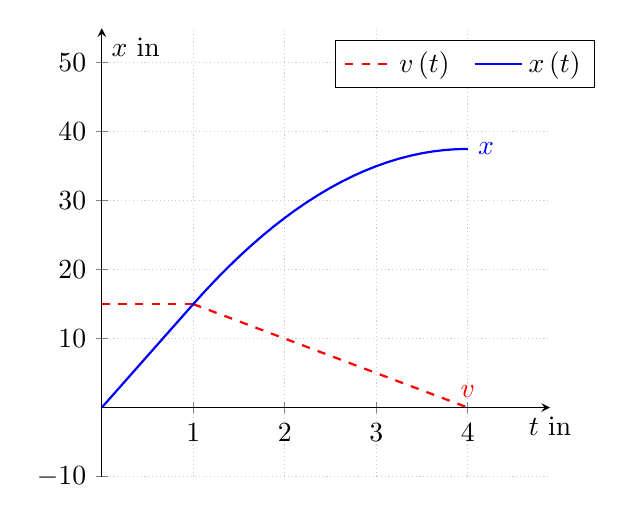
\begin{tikzpicture}
				\begin{axis}[
					width=207pt,
					height=207pt,
					axis lines=center,
%					axis line style={Stealth-Stealth},
					xmin=0,xmax=4.9,ymin=-10,ymax=55,
					xlabel style={below},
					xtick distance=1,
					ytick distance=10,
					xlabel=$t$ in\si{\s},
					ylabel=$x$ in\si{\m},
					grid=major,
					grid style={thin,densely dotted,black!20},
					legend columns=2,
					legend style={at={(axis description cs:1.1,0.92)},anchor=east}]
					\addplot [-, thick, dashed, red]
					coordinates { (0,15) (1, 15)};
					\addplot [-, thick, dashed, red, forget plot]
					coordinates { (1, 15) (4, 0)} node[above,pos=1] {$v$};
					\addplot [-, thick, blue, forget plot]	
					coordinates { (0,0) (1, 15)};
					\addplot [-, thick,  blue, domain = 1:4] 
					{-2.5*x^2 + 20*x - 2.5} node[right,pos=1] {$x$};	
					\legend{$ v\left(t\right)$~~~,$ x\left(t\right) $}
				\end{axis}
			\end{tikzpicture}\\
			\columnbreak
			\begin{enumerate}
			\item
			\begin{align*}
				v(t) &= \begin{cases}
					15 & \quad $für $\ \ 0 \le t < 1, \\
					-5t + 20 & \quad $für $\ \ 1 \le t \le 4.
				\end{cases}
			\end{align*}
			\item
			\begin{align*}
				x(t) &= \begin{cases}
					15t& \quad $für $\ 0 \le t < 1, \\
					-2.5t^2 + 20t - 2.5& \quad $für $\ 1 \le t \le 4, \\
				\end{cases}
			\end{align*}
			\item $ t_2 = \dl{4 \si{\s}}; \quad x_2 = \dl{37.5 \si{\m}}$
			\end{enumerate}
		\end{multicols}

\newpage
	\section*{13. Fahrstuhl}
		\begin{multicols}{2}
				\begin{enumerate}
					\item $ s_1 = x(2) - x(0) = \dl{4 \si{\m}} $\\
					\item $ s_2 = x(9) - x(2) = \dl{28 \si{\m}} $\\
					\item $ s_3 = x(11) - x(9) = \dl{4 \si{\m}} $\\[2ex]
					\item $ \dfrac{s_1 + s_2 + s_3}{4} + 3 = \dl{12\ \text{ Stockwerke}} $
				\end{enumerate}
			\columnbreak
			\begin{align*}
			a(t) &= \begin{cases}
				2& \quad $für $\ 0 \le t \le 2, \\
				0& \quad $für $\ 2 < t \le 9, \\
				-2& \quad $für $\ 9 < t \le 11.
			\end{cases} \\
			v(t) &= \begin{cases}
				2t& \quad $für $\ 0 \le t \le 2, \\
				4& \quad $für $\ 2 < t \le 9, \\
				-2t + 22& \quad $für $\ 9 < t \le 11.
			\end{cases} \\
			x(t) &= \begin{cases}
				t^2& \quad $für $\ 0 \le t \le 2, \\
				4t - 4& \quad $für $\ 2 < t \le 9, \\
				-t^2 + 22t - 85& \quad $für $\ 9 < t \le 11.
			\end{cases} \\
			\end{align*}
		\end{multicols}
\end{document} 